% ---------------------------------------------------------------------------
\section{Comparing new lookout with the older version (SK)} \label{sec:comparewitholderversion}
% ---------------------------------------------------------------------------
Next we compare the old and the new versions of lookout. We conduct 4 experiments that explore different aspects of the updated algorithm and illustrate the output using a set of showcase examples.  Experiments 1 and 2 consider the anomalous distribution moving away from the non-anomalous distribution and investigate the resulting performance. Experiments 3 and 4 are about increasing the number of data points in the experiment.


% - Show anomaly detection examples using normal distribution and gamma distribution, with lookout 2 vs lookout 1

\subsection{Experiment 1:  Different anomaly rates for Gamma distribution}
Consider the  $\text{Gamma}(\alpha, \beta)$ distribution with shape $\alpha$ and rate $\beta$. Experiment 1 considers the Gamma distribution with different rates $\beta$.  We select $\text{Gamma}(2, 2)$ as the non-anomalous distribution and $\text{Gamma}(2, r)$  as the anomalous distribution where $r$ changes with each iteration of the experiment with $r \in \{0.1, 0.2, \ldots, 1\}$. We let $X_i \in \mathbb{R}^2$ with $X_i = (X_{i1}, X_{i2})$ where $X_{i1}, X_{i2} \sim \text{Gamma}(2, \beta)$ for the respective rate parameters for anomalous and non-anomalous distributions. We consider 500 non-anomalies and 10 anomalies in each iteration. Each iteration is repeated 10 times to account for randomness.

\begin{figure}[!ht]
	\centering
	% 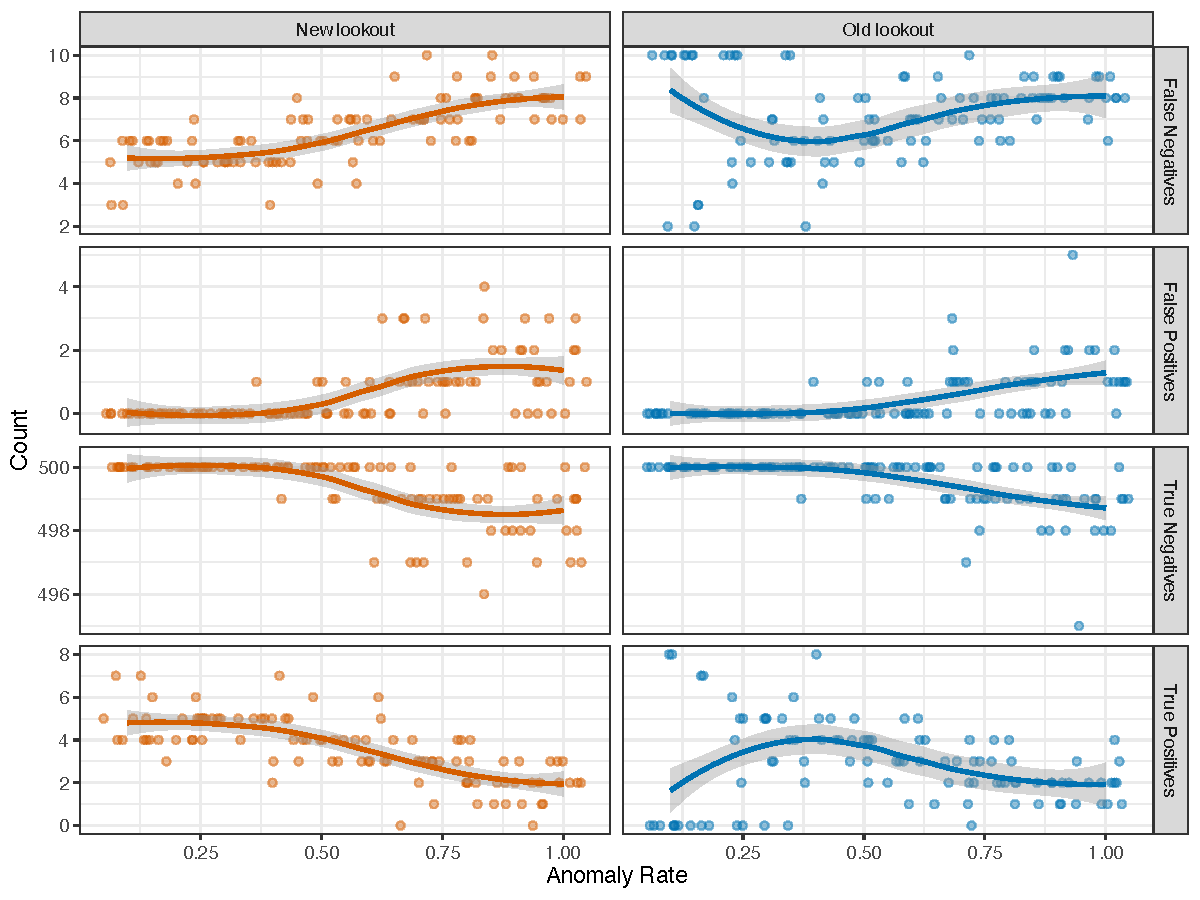
\includegraphics[width=0.8\textwidth]{Figures/EXP1_Gamma_Raw.pdf}
	% \caption{Results of the Gamma Experiment - Raw numbers.}
	% \label{fig:exp1GammaRaw}
	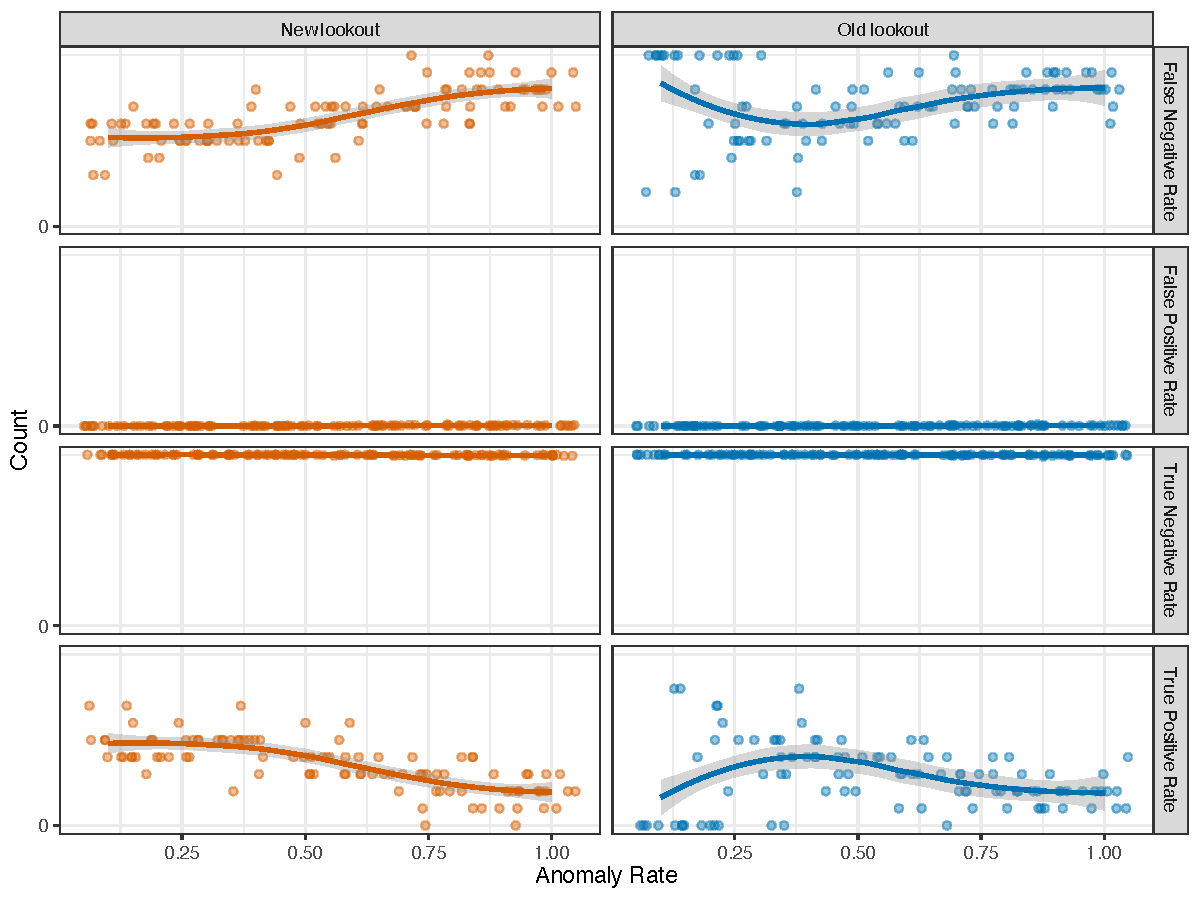
\includegraphics[width=0.8\textwidth]{Figures/EXP1_Gamma_Rates.pdf}
	\caption{Results of Experiment 1.}
	\label{fig:exp1GammaRates}
\end{figure}

Figure \ref{fig:exp1GammaRates}  shows the results of Experiment 1. As the rate $r$ of the anomalous Gamma distribution increases, the anomalies and non-anomalies become similar. Thus, we expect a decrease in the true positive rate and an increase in the false negative rate as $r$ increases. The anomalies are most different from non-anomalies when $r = 0.1$. We see that new lookout performs better for these cases compared to the old version. Old lookout oscillates between high and low performances for $r = 0.1$, whereas the new version consistently performs well.

\subsection{Experiment 2:  Different anomaly rates for Normal distribution}

Next we consider the normal distribution $\mathcal{N}(\mu, \sigma)$ with mean $\mu$ and standard deviation $\sigma$. As before we consider separate $\mu$ and $\sigma$ for non-anomalous and anomalous distributions. We let $X_i = (X_{i1}, X_{i2}) \in \mathbb{R}^2$ with $X_{i1}, X_{i2} \sim \mathcal{N}(\mu, \sigma)$. The non-anomalous distribution is  $\mathcal{N}(0, 1)$. The anomalous distribution has $\mu \in \{ 2.50, 2.75,  3.00 , 3.25,  3.50, 3.75, 4.00\} $ and $\sigma = 0.2$. We consider 1000 non-anomalies and 10 anomalies and repeat every iteration (for each $\mu$) 10 times.

\begin{figure}[!ht]
	\centering
	% 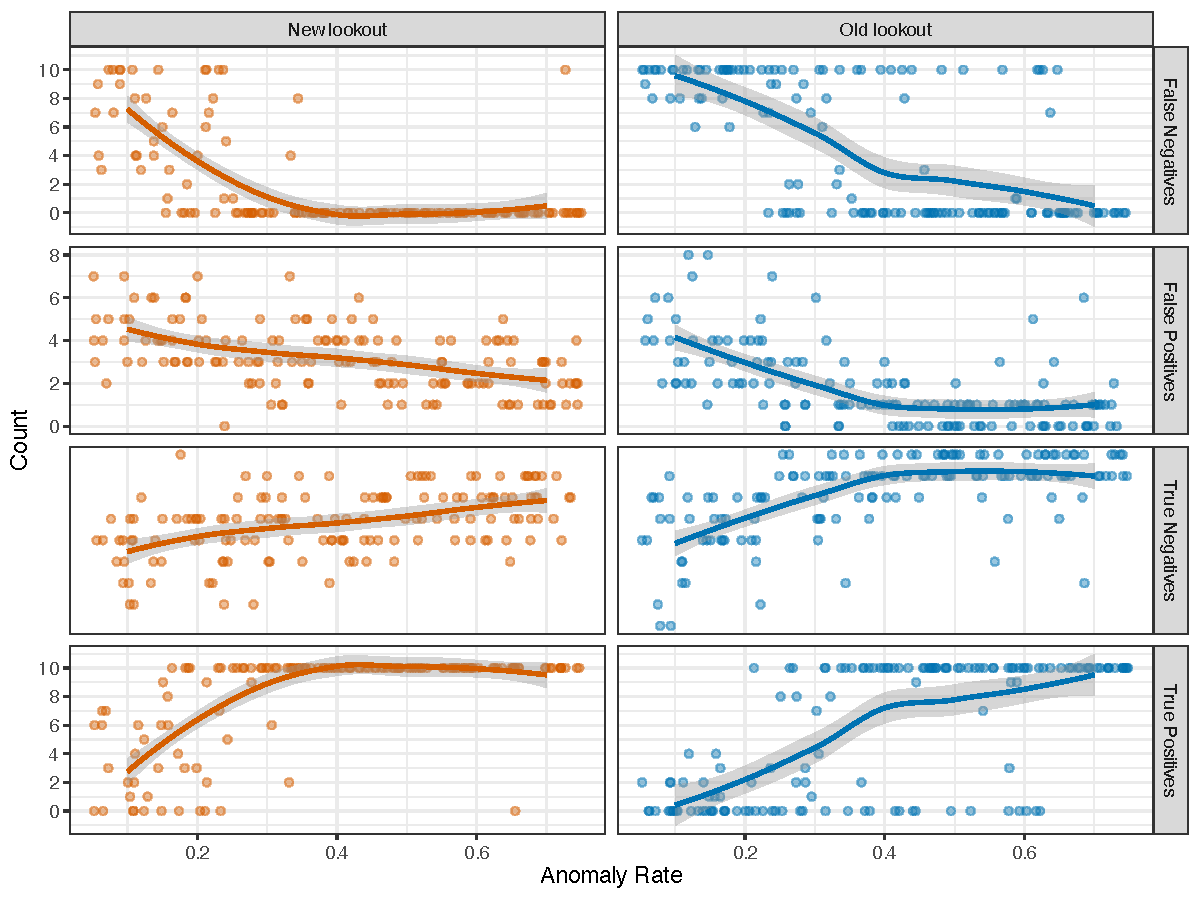
\includegraphics[width=0.8\textwidth]{Figures/EXP2_Normal_Raw.pdf}
	% \caption{Results of the Normal Dist. Exp. - Raw numbers.}
	% \label{fig:exp2NormalRaw}
	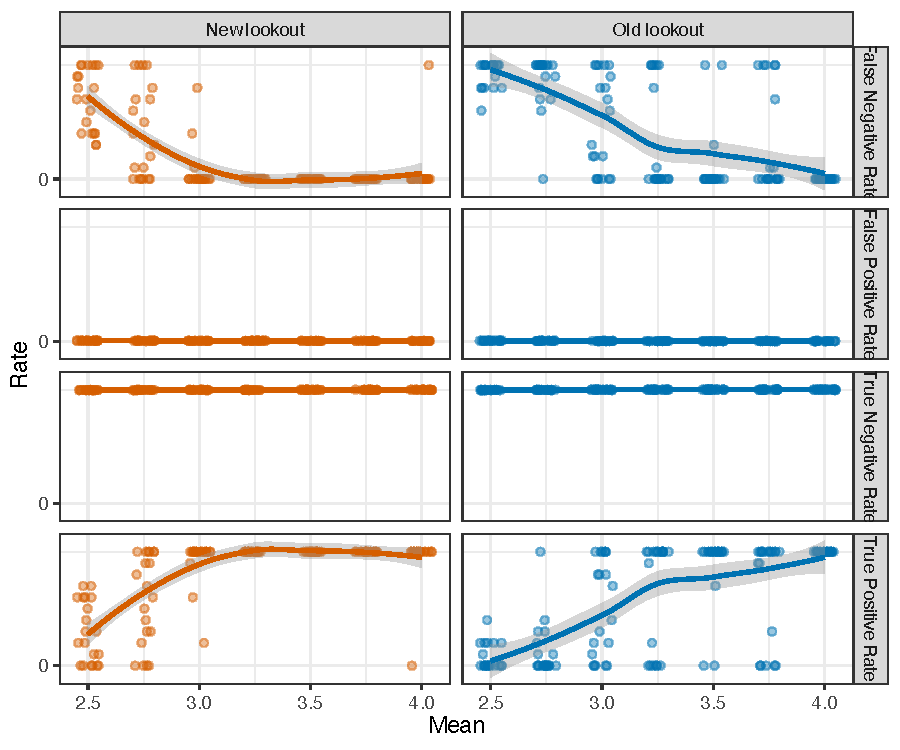
\includegraphics[width=0.7\textwidth]{Figures/EXP2_Normal_Rates.pdf}
	\caption{Results of the Experiment 2.}
	\label{fig:exp2NormalRates}
\end{figure}

Figure \ref{fig:exp2NormalRates} shows Experiment 2 results. As $\mu$ increases, the anomalies shift away from the non-anomalies. Thus, we expect the true positive rate to increase and the false negative rate to decrease with $\mu$. Again new lookout performs better than old lookout, achieving higher true positive rates as well as lower false negative rates sooner with increasing $\mu$.

% Non-outlier distribution: 1000 data points in $\mathbb{R}^2$, mean = $(0,0)$,  standard deviation = 1 \\
% Outlier distribution: 10 data points,  mean $\in \{ 2.50, 2.75,  3.00 , 3.25,  3.50, 3.75, 4.00\}$ standard deviation = 0.2.

% For the normal distribution -- False positives are slightly higher with the new version. But true positives are better.

% \SK{For Experiments 1 and 2 (Gamma and Normal experiments), I've put both graphs, one with false positives and the other with false positive rates. We need to choose one of these graphs. I prefer the rates because 6 or 4 false positives doesn't really make a difference when there are 1000 data points. Similarly for true negatives. But 6 true positives (or false negatives) are different from 4 true positives when there are only 10 anomalies.   }

% \begin{figure}[!p]
%   \centering
%   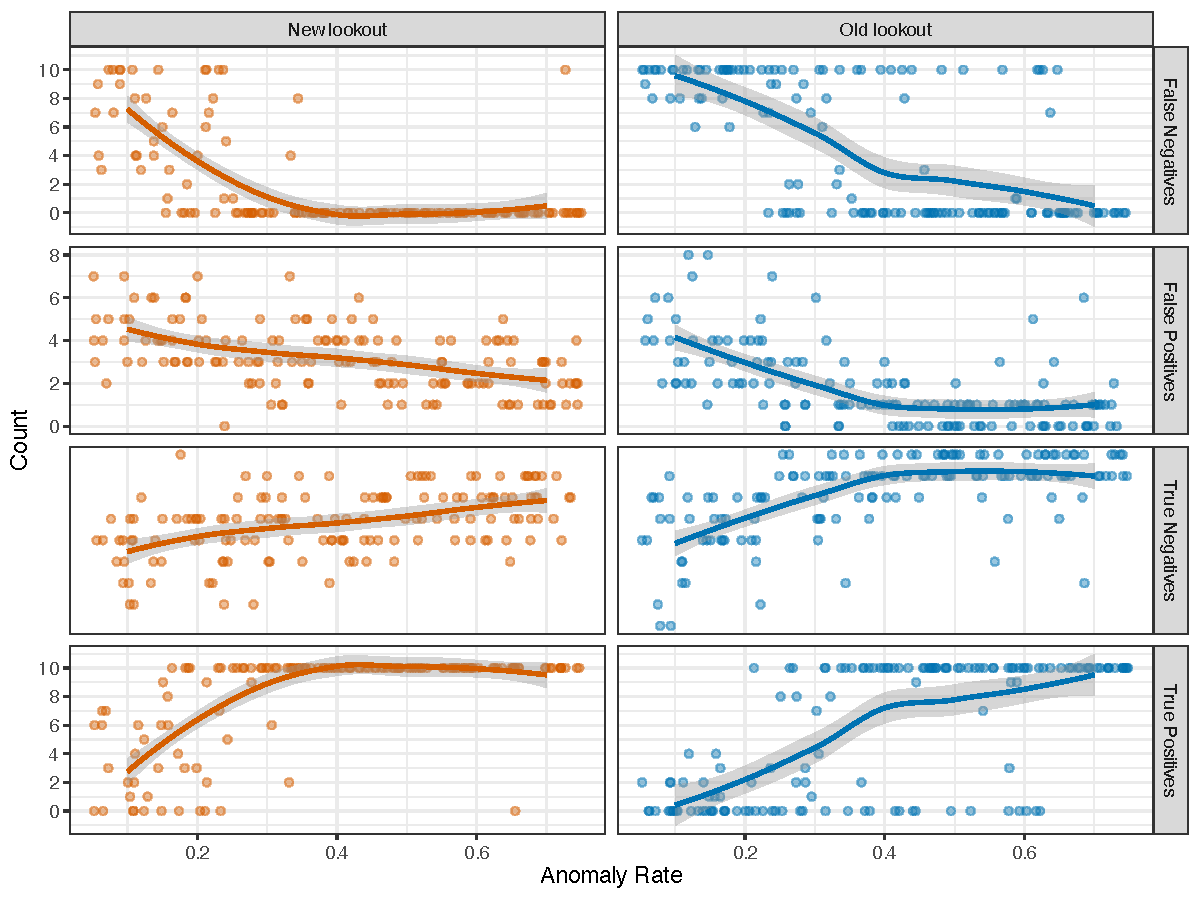
\includegraphics[width=0.8\textwidth]{Figures/EXP2_Normal_Raw.pdf}
%   \caption{Results of the Normal Dist. Exp. - Raw numbers.}
%   \label{fig:exp2NormalRaw}
%   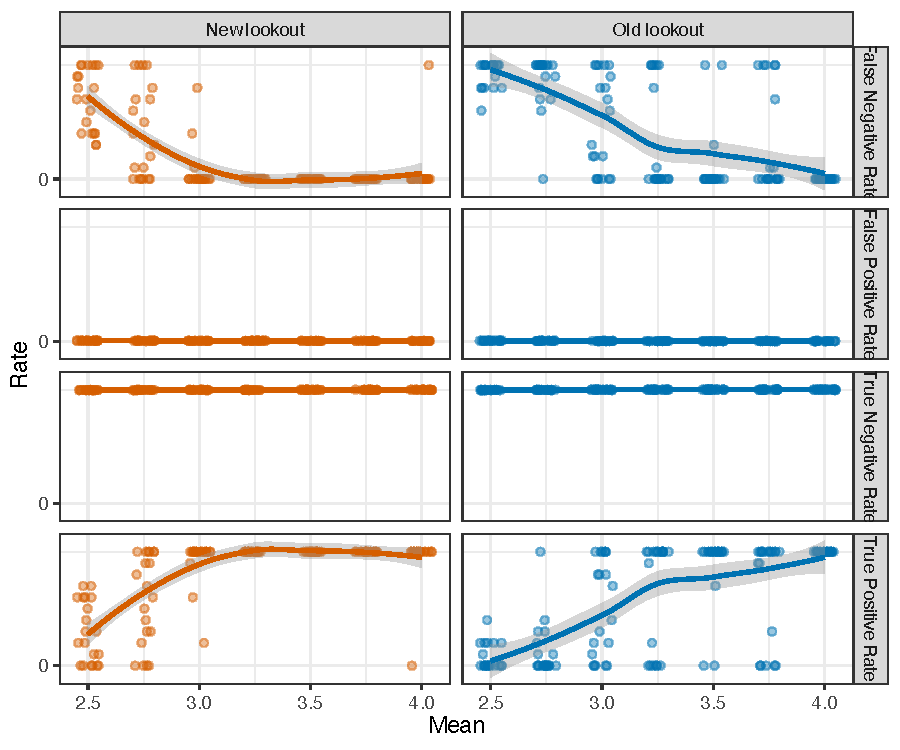
\includegraphics[width=0.8\textwidth]{Figures/EXP2_Normal_Rates.pdf}
%   \caption{Results of the Normal Dist. Exp. - Rates.}
%   \label{fig:exp2NormalRates}
% \end{figure}


\subsection[Experiment 3: As N increases - Normal distribution]{Experiment 3: As $N$ increases - Normal distribution}
We consider $X_i = (X_{i1}, X_{i1}) \in \mathbb{R}^2$ with $X_{i1}, X_{i2} \sim \mathcal{N}(\mu, \sigma)$ with $\mu = 0$ and $\sigma = 1$ for non-anomalies  and $\mu = 2.2$ and $\sigma = 0.2$ for anomalies. We consider $n$ non-anomalies for $n \in \{1000, 2000, \ldots, 10000\}$ and 5 anomalies. Each iteration for a given $n$ is repeated 10 times.

\begin{figure}[!ht]
	\centering
	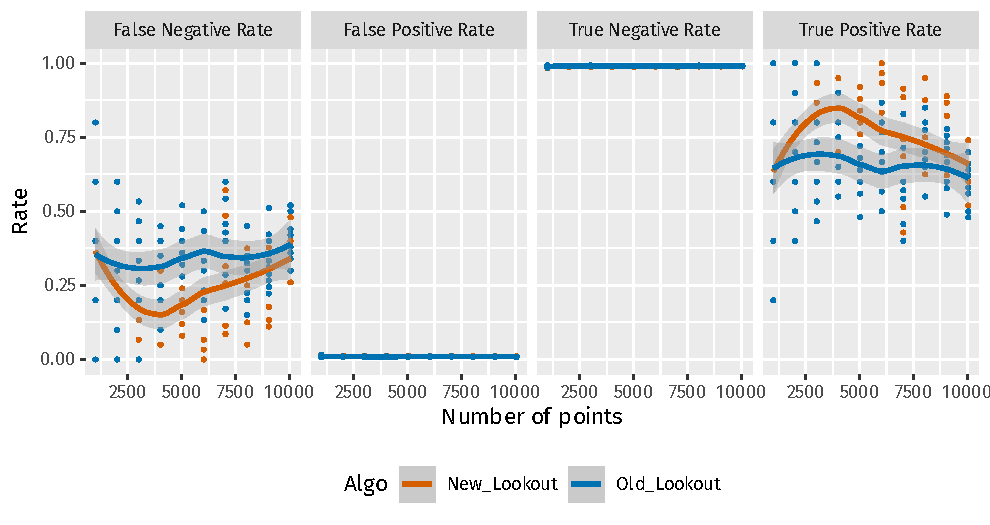
\includegraphics[width=0.9\linewidth]{Figures/Exp3_N_Increases_Normal.pdf}
	\caption{Experiment 3 results.}
	\label{fig:exp3NormalIncreasingN}
\end{figure}

Figure \ref{fig:exp3NormalIncreasingN} shows the results of Experiment 3. Both new and old lookout give low false positive rates and high true negative rates. However, we see that new lookout has a larger true positive rate and a lower false negative rate compared to old lookout demonstrating that it performs better.

% Non-outlier distribution: $N \in \{1000, 2000, \ldots, 10000\}$, mean =0, sd = 1 \\
% Outlier distribution: 5 points mean = 2.2, sd = 0.2 \\
% Both non-outlier and outlier distributions are Normal.

\begin{figure}[!ht]
	% \centering
	% 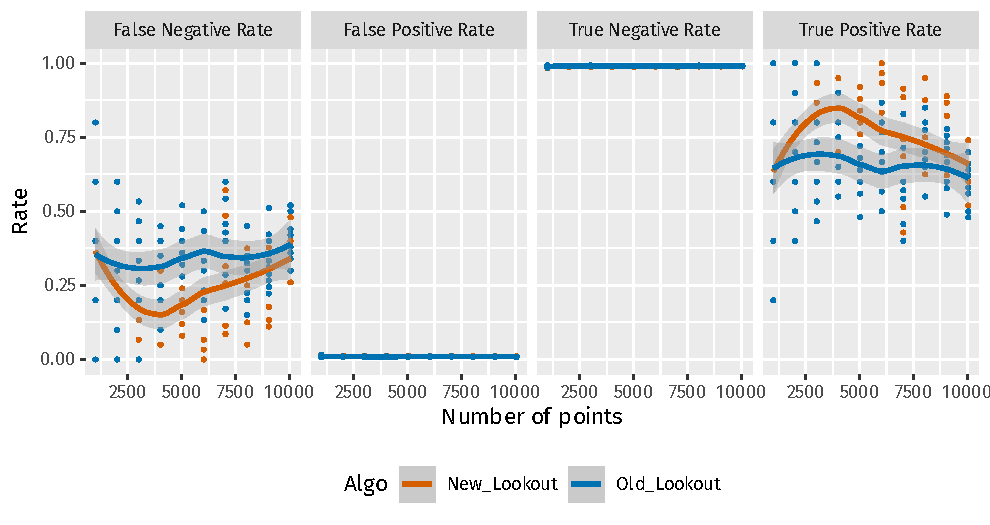
\includegraphics[width=0.9\linewidth]{Figures/Exp3_N_Increases_Normal.pdf}
	% \caption{Experiment 3 results - Normal distribution}
	% \label{fig:exp3NormalIncreasingN}
	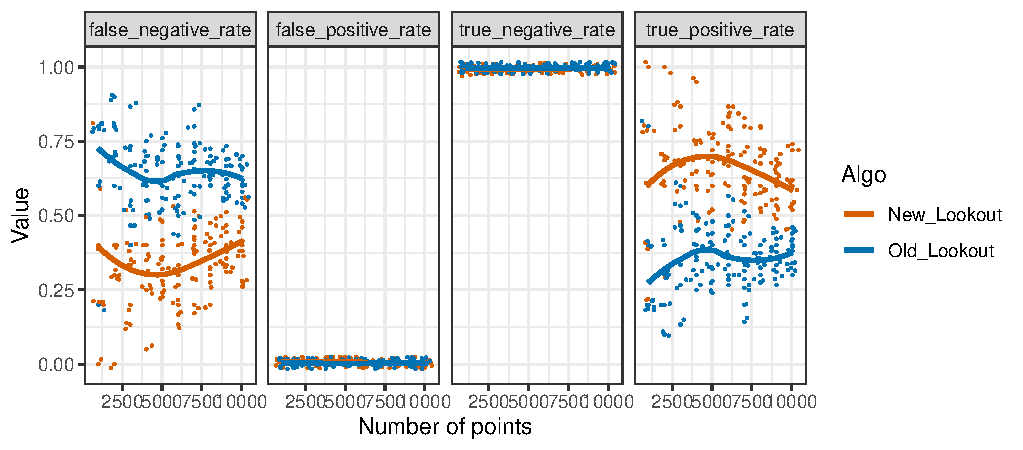
\includegraphics[width=0.9\linewidth]{Figures/EXP4_N_increases_Gamma.pdf}
	\caption{Experiment 4 results - Gamma and Normal distributions}
	\label{fig:exp4GammaIncreasingN}
\end{figure}

\subsection[Experiment 4: As N increases - Gamma + Normal distributions]{Experiment 4: As $N$ increases - Gamma + Normal distributions}
For this experiment we consider $X_i \in \mathbb{R}^2$ with $X_i = (X_{i1}, X_{i2})$.  The non-anomalies  $X_{i1}, X_{i2} \sim \text{Gamma}(2, 2)$ and the anomalies $X_{i1}, X_{i2} \sim  \mathcal{N}(3, 0.5)$. There are $n$ non-anomalies and $5$ anomalies with $n \in \{1000, 2000, \ldots, 10000\}$ in each iteration. Figure \ref{fig:exp4GammaIncreasingN} shows the results and as before we see new lookout performs better.

% Non-outlier distribution: Gamma with $N \in \{1000, 2000, \ldots, 10000\}$, shape =2, rate = 2 \\
% Outlier distribution: Normal 5 points with mean = $(3,3)$, sd = 0.5. \\
% Outlier distribution is normal, while non-outlier distribution is Gamma.


\subsection{Showcase examples}
\begin{figure}[!p]
	\centering
	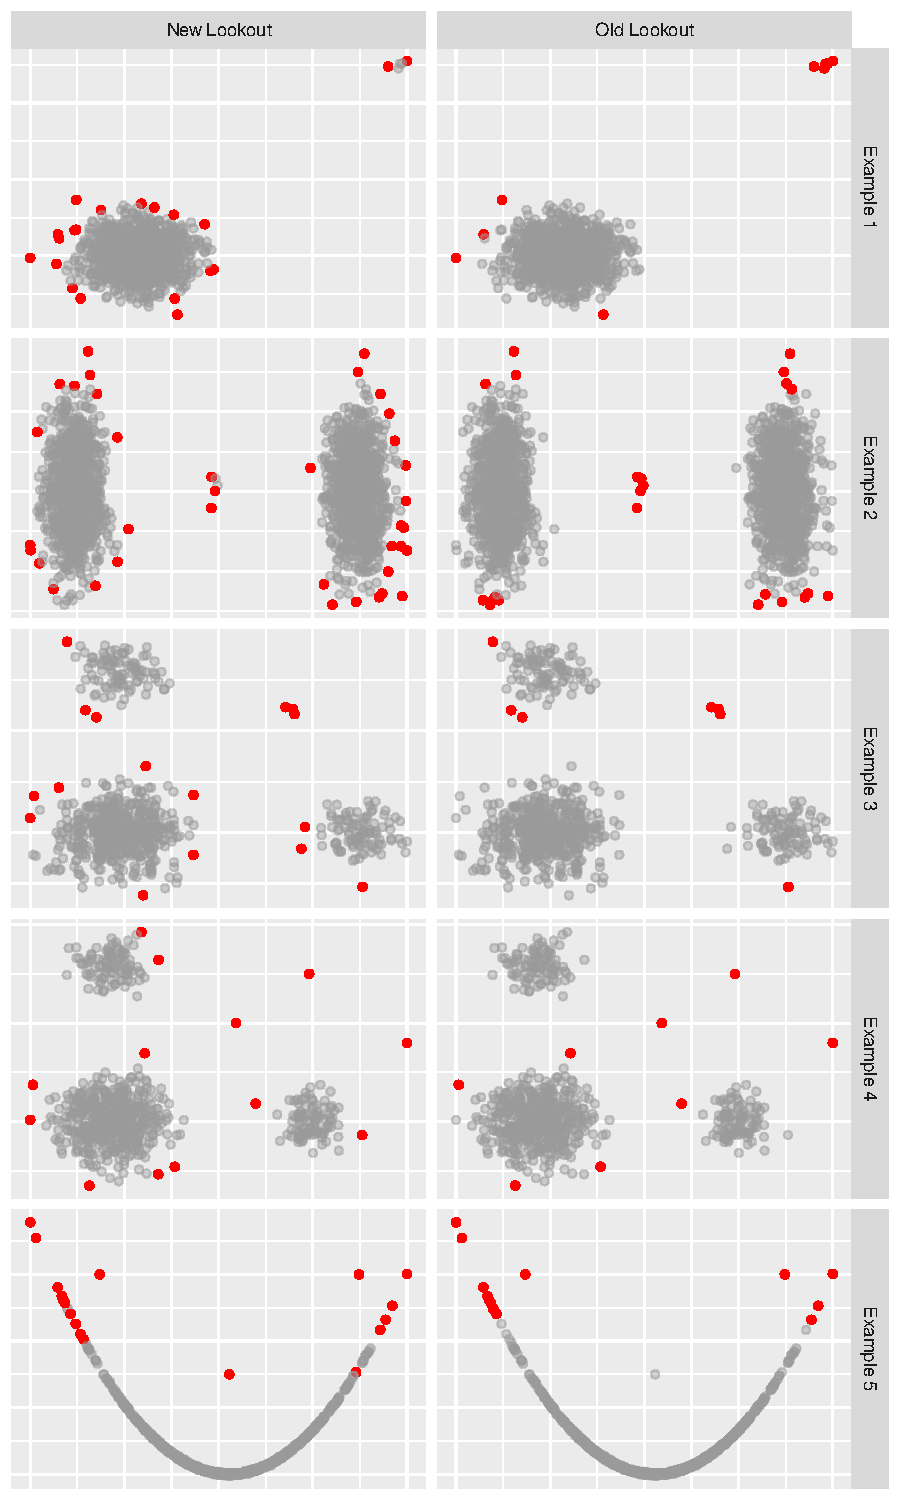
\includegraphics[width=0.84\linewidth]{Figures/Showcase_Examples.pdf}
	\caption{Comparing new lookout with the older version on some showcase examples}
	\label{fig:showcaseExamples}
\end{figure}
\clearpage
